\chapter{Requisitos del Software}

Una vez realizada la introducción, donde se ha descrito de qué trata el proyecto y qué se va a
desarrollar, en este capítulo se lleva a cabo un estudio de la ingeniería de requisitos que permite
realizar una descripción funcional del sistema. En primer lugar se describe el perfil de los
usuarios, ya que los requisitos se refieren a ellos y conviene tener claro qué puede hacer cada uno;
a continuación se detallan los requisitos (funcionales, no funcionales y de información), los casos
de uso y, por último, la asignación de los requisitos a los sprints y los criterios de validación.

\section{Perfil de usuarios}

Se denominará \textbf{usuario} al conjunto de personas que utilicen la aplicación. La aplicación está
dirigida a personas interesadas en explorar y analizar redes cerebrales, y se distinguen tres grupos
de roles. Para referirse a ellos de forma abreviada se emplean las siglas \textbf{[V]} (visitante),
\textbf{[I]} (investigador) y \textbf{[A]} (administrador):

\begin{description}
	\item[\textbf{[V] Visitante.}] Accede a la aplicación sin necesidad de registro. Puede explorar
		las redes cerebrales públicas precargadas: visualizarlas en 3D, navegar, filtrar, inspeccionar
		nodos, consultar métricas y personalizar la vista. No puede subir ni almacenar datos.
	\item[\textbf{[I] Investigador.}] Usuario registrado. Además de todo lo anterior, puede cargar sus
		propias redes cerebrales, gestionar sus \textit{conjuntos de datos} privados y exportar los
		resultados (visualizaciones y métricas).
	\item[\textbf{[A] Administrador.}] Rol único de moderación. Además de todo lo anterior, gestiona el
		catálogo de redes públicas disponibles para todos (altas, ediciones y bajas) y gestiona los
		usuarios del sistema: da de alta y de baja usuarios y les asigna o revoca el rol de
		investigador.
\end{description}

De igual forma que en otros sistemas con roles, las funciones de cada rol se ven recogidas y
ampliadas (herencia) por el rol de mayor relevancia, siendo el orden principal \textbf{Administrador
-- Investigador -- Visitante}. Es decir, el investigador puede hacer todo lo que hace un visitante, y
el administrador todo lo que hace un investigador, más sus funciones específicas.

\section{Requisitos}

A continuación se describen las funcionalidades de la aplicación. En primer lugar, los requisitos
funcionales, es decir, las funciones de la aplicación cuando el usuario la utiliza; se distinguen
funcionalidades generales y funcionalidades propias de cada rol. En segundo lugar, los requisitos no
funcionales, que recogen aspectos de rendimiento, seguridad y usabilidad. Por último, los requisitos
de información, que describen los datos que el sistema debe almacenar y gestionar.

Cada requisito se prioriza, ya que los requisitos se implementan por \textit{sprints} en orden de
prioridad: si al finalizar el proyecto no se llegaran a implementar todos, los pendientes serían
siempre los de menor prioridad. La prioridad~1 identifica los requisitos que constituyen el
\textbf{producto mínimo viable} (o MVP, del inglés \textit{Minimum Viable Product}): el conjunto
mínimo de funcionalidades sin las cuales el sistema no sería viable. La tabla~\ref{tab:prioridades}
recoge la correspondencia entre el nivel de prioridad y el sprint en el que se implementa.

\begin{table}[H]
	\centering
	\caption{Niveles de prioridad de los requisitos funcionales.}
	\label{tab:prioridades}
	\begin{tabularx}{\textwidth}{>{\centering\arraybackslash}p{2.2cm} l >{\centering\arraybackslash}p{1.8cm} >{\raggedright\arraybackslash}X}
		\toprule
		\textbf{Prioridad} & \textbf{Nivel} & \textbf{Sprint} & \textbf{Significado} \\
		\midrule
		1 & Crítica & 1 & Imprescindible; constituye el producto mínimo viable del sistema. \\
		2 & Alta    & 2 & Aporta el valor principal de exploración interactiva. \\
		3 & Media   & 3 & Análisis de red; distingue la herramienta de un simple visor. \\
		4 & Baja    & 4 & Cuentas de usuario, gestión de datos y administración. \\
		\bottomrule
	\end{tabularx}
\end{table}

\subsection{Requisitos funcionales}

\subsubsection*{Funcionalidades generales (rol visitante [V] o superior)}

\noindent\textbf{[RF 1]} Cualquier usuario podrá acceder a la aplicación y explorar las redes
cerebrales públicas precargadas sin necesidad de registro, actuando como visitante [V].

\noindent\textbf{[RF 2]} El usuario podrá visualizar la red cerebral seleccionada renderizada en un
espacio 3D interactivo, con los nodos situados en sus coordenadas anatómicas y las aristas ponderadas
entre ellos.
\begin{itemize}
	\item \textbf{[RF 2.1]} El sistema procesará en el servidor los ficheros de la red (nodos y matriz
		de adyacencia), construirá el grafo y lo pondrá a disposición del cliente a través de una
		interfaz de programación (API).
\end{itemize}

\noindent\textbf{[RF 3]} El usuario podrá navegar por la escena mediante controles de cámara orbital:
rotar, hacer zoom y desplazar (paneo).

\noindent\textbf{[RF 4]} El usuario dispondrá de un panel de estadísticas globales (HUD) con el
número de nodos, aristas y grupos de la red activa.

\noindent\textbf{[RF 5]} El usuario podrá filtrar dinámicamente las aristas visibles mediante un
umbral de peso ajustable en tiempo real.

\noindent\textbf{[RF 6]} El usuario podrá seleccionar un nodo haciendo clic sobre él, que quedará
resaltado, y consultar su información detallada (etiqueta, coordenadas, grado y grupo).
\begin{itemize}
	\item \textbf{[RF 6.1]} La información del nodo se ampliará con sus métricas de centralidad
		(grado, intermediación y cercanía).
\end{itemize}

\noindent\textbf{[RF 7]} El usuario podrá colorear los nodos según su grupo o lóbulo anatómico, con
una leyenda de colores asociada.

\noindent\textbf{[RF 8]} El usuario podrá consultar las métricas globales de la red (densidad, grado
medio, coeficiente de \textit{clustering} y número de componentes conexas), calculadas en el
servidor.

\noindent\textbf{[RF 9]} El usuario podrá cambiar el criterio visual de los nodos, haciendo que su
tamaño o color dependa de una métrica seleccionada.

\noindent\textbf{[RF 10]} El usuario podrá buscar un nodo por su etiqueta y el sistema centrará la
cámara sobre él.

\noindent\textbf{[RF 11]} El usuario podrá personalizar la visualización (tamaño de nodos, opacidad
de aristas, ejes de referencia, rotación automática y tema) y restablecerla a su estado inicial.

\noindent\textbf{[RF 12]} El usuario podrá exportar la visualización actual como imagen.

\subsubsection*{Funcionalidades del rol investigador [I]}

\noindent\textbf{[RF 13]} Un investigador podrá registrarse e iniciar sesión para acceder a las
funcionalidades de gestión de datos.

\noindent\textbf{[RF 14]} Un investigador podrá cargar sus propias redes cerebrales mediante la
subida simultánea de los dos ficheros que describen una red: uno con las coordenadas y los atributos
de los nodos, y otro con la matriz de conexiones (definidos en [RI 1] y [RI 2]).
\begin{itemize}
	\item \textbf{[RF 14.1]} El sistema validará el formato y la consistencia dimensional de los
		ficheros antes de cargar la red, informando de cualquier error.
\end{itemize}

\noindent\textbf{[RF 15]} Un investigador podrá gestionar sus propios conjuntos de datos: guardarlos,
listarlos y eliminarlos.

\noindent\textbf{[RF 16]} Un investigador podrá exportar las métricas calculadas de una red en un
formato de intercambio de datos.

\subsubsection*{Funcionalidades del rol administrador [A]}

\noindent\textbf{[RF 17]} Un administrador podrá gestionar el catálogo de redes públicas, añadiendo,
editando o eliminando las redes precargadas disponibles para todos los usuarios.

\noindent\textbf{[RF 18]} Un administrador podrá gestionar los usuarios registrados: consultarlos,
editar su rol o eliminarlos.
\begin{itemize}
	\item \textbf{[RF 18.1]} El administrador podrá asignar o revocar el rol de investigador a un
		usuario.
\end{itemize}

\vspace{0.4cm}
La tabla~\ref{tab:priorizacion} resume todos los requisitos funcionales, el rol mínimo que puede
ejecutarlos y su prioridad.

\begin{table}[H]
	\centering
	\caption{Priorización de los requisitos funcionales.}
	\label{tab:priorizacion}
	\small
	\begin{tabularx}{\textwidth}{>{\centering\arraybackslash}p{1.4cm} >{\raggedright\arraybackslash}X >{\raggedright\arraybackslash}p{2.6cm} >{\centering\arraybackslash}p{1.4cm}}
		\toprule
		\textbf{RF} & \textbf{Resumen de funcionalidad} & \textbf{Rol mínimo} & \textbf{Prior.} \\
		\midrule
		RF 1  & Acceso como visitante y exploración de redes públicas. & Visitante & 1 \\
		RF 2  & Visualización 3D de la red (nodos y aristas). & Visitante & 1 \\
		RF 2.1 & Procesamiento en el servidor y exposición mediante una API. & Visitante & 1 \\
		RF 3  & Navegación con cámara orbital. & Visitante & 1 \\
		RF 4  & Panel de estadísticas globales (HUD). & Visitante & 1 \\
		\addlinespace
		RF 5  & Filtrado de aristas por umbral de peso. & Visitante & 2 \\
		RF 6  & Selección e inspección de un nodo. & Visitante & 2 \\
		RF 7  & Coloreado de nodos por grupo/lóbulo. & Visitante & 2 \\
		\addlinespace
		RF 6.1 & Métricas de centralidad por nodo. & Visitante & 3 \\
		RF 8  & Métricas globales de la red (en el servidor). & Visitante & 3 \\
		RF 9  & Mapeo visual de métricas (tamaño/color). & Visitante & 3 \\
		RF 10 & Búsqueda de nodo por etiqueta. & Visitante & 3 \\
		\addlinespace
		RF 11 & Personalización y restablecimiento de la vista. & Visitante & 4 \\
		RF 12 & Exportación de la vista como imagen. & Visitante & 4 \\
		RF 13 & Registro e inicio de sesión. & Investigador & 4 \\
		RF 14 & Carga de redes propias. & Investigador & 4 \\
		RF 14.1 & Validación de los ficheros cargados. & Investigador & 4 \\
		RF 15 & Gestión de conjuntos de datos propios. & Investigador & 4 \\
		RF 16 & Exportación de métricas. & Investigador & 4 \\
		RF 17 & Gestión del catálogo de redes públicas. & Administrador & 4 \\
		RF 18 & Gestión de usuarios. & Administrador & 4 \\
		RF 18.1 & Asignación/revocación del rol investigador. & Administrador & 4 \\
		\bottomrule
	\end{tabularx}
\end{table}

\subsection{Requisitos no funcionales}

\noindent\textbf{[RNF 1]} La aplicación deberá garantizar un rendimiento gráfico fluido en la
manipulación del modelo 3D, apoyándose en la aceleración gráfica por hardware, con una tasa de
fotogramas estable (objetivo: $\geq 60$~FPS con redes de hasta unos 500 nodos y $\geq 30$~FPS hasta
unos 1000 nodos).

\noindent\textbf{[RNF 2]} La aplicación deberá garantizar la confidencialidad de los datos: los
conjuntos de datos privados de un investigador solo serán accesibles por él mismo y por el
administrador. Ningún otro usuario podrá acceder a la información privada de otro.

\noindent\textbf{[RNF 3]} La aplicación deberá avisar al usuario cuando surja algún tipo de error que
no dependa de él (por ejemplo, dimensiones incongruentes entre los ficheros de entrada), siendo lo
más transparente posible en cada caso e indicando qué falla y por qué.

\noindent\textbf{[RNF 4]} La interfaz de navegación deberá ser suficientemente intuitiva para que
cada usuario sepa en cada momento cómo interactuar con el modelo 3D y qué está visualizando, sin
necesidad de una fuente de información externa.

\noindent\textbf{[RNF 5]} El sistema deberá empaquetarse en contenedores y poder levantarse con un
único comando, garantizando la reproducibilidad del entorno con independencia del sistema operativo
anfitrión.

\noindent\textbf{[RNF 6]} La aplicación deberá funcionar en los navegadores web modernos más
habituales, sin necesidad de instalar complementos adicionales.

\subsection{Requisitos de información}

\noindent\textbf{[RI 1]} El documento para introducir la topología de los nodos debe ser un fichero
de texto plano con las columnas \texttt{x  y  z  color\_id  size  label}, siendo obligatorias las
coordenadas $(x, y, z)$ y opcionales el identificador de grupo, el tamaño y la etiqueta; el separador
es uno o más espacios o tabuladores. Este formato sigue la convención de \textit{BrainNet
Viewer}~\cite{brainnet}.

\noindent\textbf{[RI 2]} El documento para introducir las conexiones debe ser un fichero de texto
plano que contenga una matriz de adyacencia cuadrada $N \times N$. Cada valor representa el peso de
la conexión entre dos nodos, siendo \textbf{0} la ausencia de conexión; los pesos son valores
numéricos y no se asume que estén normalizados. La matriz será simétrica (grafo no dirigido) y con
diagonal a cero.

\noindent\textbf{[RI 3]} Cualquier dato introducido a través de los ficheros o formularios de la
aplicación deberá recogerse en formato de codificación estándar UTF-8.

\noindent\textbf{[RI 4]} La aplicación deberá almacenar de forma consistente y privada los datos de
cada entidad que interactúe con el sistema.
\begin{itemize}
	\item \textbf{[RI 4.1]} De cada usuario se almacenará su identificador, sus credenciales y su rol;
		solo podrán ser modificados por el propio usuario o por un administrador.
	\item \textbf{[RI 4.2]} De cada conjunto de datos se almacenará su nombre, su propietario, su
		visibilidad (público o privado) y los ficheros de la red asociada.
\end{itemize}

\section{Casos de uso}

En este apartado se describen los casos de uso de la aplicación desde la perspectiva de los usuarios
que interactúan con ella de forma directa. En una primera fase se presentan los diagramas de casos
de uso, que ofrecen una representación gráfica de la relación entre los casos de uso y los
participantes (denominados \textit{actores}). Posteriormente se realiza una descripción detallada de
los pasos, acciones y resultados esperados de cada caso de uso.

Se emplean las siguientes siglas para abreviar:
\begin{itemize}
	\item \textbf{CU:} Caso de Uso.
	\item \textbf{Diagrama CU:} Diagrama de Caso de Uso.
	\item \textbf{CU-XX:} Caso de Uso -- número de caso de uso.
\end{itemize}

\subsection{Diagramas de casos de uso}

En las figuras~\ref{fig:cu-visitante}, \ref{fig:cu-investigador} y \ref{fig:cu-administrador} se
muestran los diagramas de casos de uso, uno por perfil de usuario. Cada diagrama recoge las tareas
que puede realizar el rol correspondiente; al existir herencia entre roles, cada diagrama incluye
implícitamente los casos de uso de los roles inferiores.

\begin{figure}[H]
	\centering
	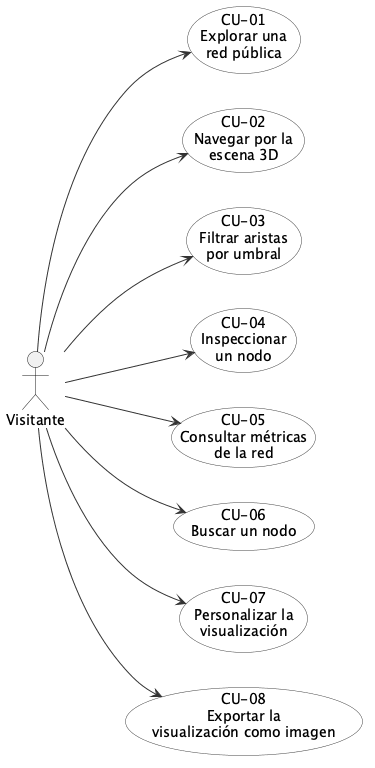
\includegraphics[height=14cm]{imagenes/cu_visitante}
	\caption{Diagrama de casos de uso del rol Visitante [V].}
	\label{fig:cu-visitante}
\end{figure}

\begin{figure}[H]
	\centering
	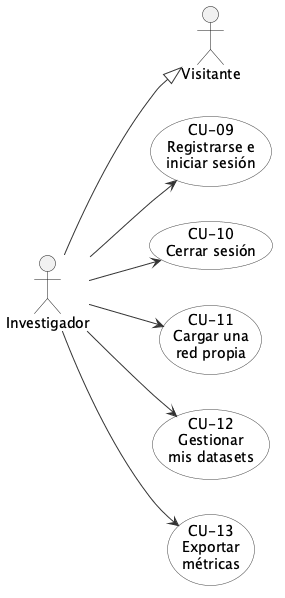
\includegraphics[height=12cm]{imagenes/cu_investigador}
	\caption{Diagrama de casos de uso del rol Investigador [I].}
	\label{fig:cu-investigador}
\end{figure}

\begin{figure}[H]
	\centering
	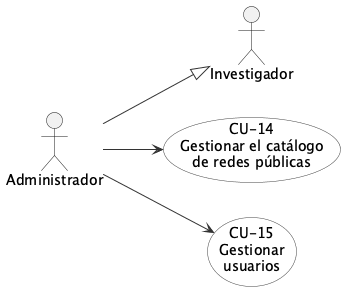
\includegraphics[height=6cm]{imagenes/cu_administrador}
	\caption{Diagrama de casos de uso del rol Administrador [A].}
	\label{fig:cu-administrador}
\end{figure}

\subsection{Descripción de los casos de uso}

Cada caso de uso se describe mediante una ficha detallada que recoge su actor, sus dependencias con
los requisitos funcionales, precondiciones, tipo, descripción, secuencia de pasos, postcondición y
excepciones (tablas~\ref{cu:01} a~\ref{cu:15}). Previamente, la tabla~\ref{tab:cu-resumen} muestra un
resumen con los casos de uso, su actor y los requisitos funcionales que implementan, poniendo de
manifiesto la trazabilidad entre requisitos y casos de uso.

\begin{table}[H]
	\centering
	\caption{Casos de uso y requisitos asociados.}
	\label{tab:cu-resumen}
	\small
	\begin{tabularx}{\textwidth}{>{\centering\arraybackslash}p{1.3cm} >{\raggedright\arraybackslash}X >{\raggedright\arraybackslash}p{2.5cm} >{\raggedright\arraybackslash}p{2.7cm}}
		\toprule
		\textbf{CU} & \textbf{Nombre} & \textbf{Actor} & \textbf{RF asociados} \\
		\midrule
		CU-01 & Explorar una red pública & Visitante & RF 2, RF 2.1 \\
		CU-02 & Navegar por la escena 3D & Visitante & RF 3 \\
		CU-03 & Filtrar aristas por umbral & Visitante & RF 5 \\
		CU-04 & Inspeccionar un nodo & Visitante & RF 6, RF 6.1 \\
		CU-05 & Consultar métricas de la red & Visitante & RF 8 \\
		CU-06 & Buscar un nodo & Visitante & RF 10 \\
		CU-07 & Personalizar la visualización & Visitante & RF 7, RF 9, RF 11 \\
		CU-08 & Exportar la visualización como imagen & Visitante & RF 12 \\
		\addlinespace
		CU-09 & Registrarse e iniciar sesión & Investigador & RF 13 \\
		CU-10 & Cerrar sesión & Investigador & RF 13 \\
		CU-11 & Cargar una red propia & Investigador & RF 14, RF 14.1 \\
		CU-12 & Gestionar mis conjuntos de datos & Investigador & RF 15 \\
		CU-13 & Exportar métricas & Investigador & RF 16 \\
		\addlinespace
		CU-14 & Gestionar el catálogo de redes públicas & Administrador & RF 17 \\
		CU-15 & Gestionar usuarios & Administrador & RF 18, RF 18.1 \\
		\bottomrule
	\end{tabularx}
\end{table}

% Fichas de casos de uso. Se usa xltabular para permitir el corte entre páginas.
% Columna 1: etiqueta del campo; Columna 2: contenido / acción.
\newcolumntype{K}{>{\raggedright\arraybackslash}p{3.3cm}}
\newcolumntype{V}{>{\raggedright\arraybackslash}X}
\setlength{\extrarowheight}{1.5pt}

% ------------------------------------------------------------------ CU-01
{\small
\begin{xltabular}{\textwidth}{|K|V|}
\caption{CU-01. Explorar una red pública.}\label{cu:01}\\
\hline
\rowcolor[gray]{0.88}\textbf{CU-01} & \textbf{Explorar una red pública} \\ \hline
\endfirsthead
\hline \rowcolor[gray]{0.88}\textbf{CU-01} & \textbf{Explorar una red pública (cont.)} \\ \hline
\endhead
\textbf{Actor principal} & Visitante [V] \\ \hline
\textbf{Dependencias} & RF 2, RF 2.1 \\ \hline
\textbf{Precondición} & La aplicación está desplegada y existe al menos una red pública disponible. \\ \hline
\textbf{Tipo} & Primario / Esencial \\ \hline
\textbf{Descripción} & El visitante selecciona una red pública y el sistema la procesa y la renderiza en 3D. \\ \hline
\rowcolor[gray]{0.88}\multicolumn{2}{|c|}{\textbf{Secuencia}} \\ \hline
\textbf{Paso} & \textbf{Acción} \\ \hline
1  & El visitante accede a la aplicación. \\ \hline
2  & El sistema muestra una red por defecto ya renderizado y la lista de redes disponibles. \\ \hline
3  & El visitante selecciona una red de la lista. \\ \hline
3a & El \textit{backend} procesa la red y la devuelve; el sistema la renderiza en 3D. \\ \hline
3b & La red no se puede cargar; se informa del error y se mantiene la anterior. \\ \hline
\textbf{Postcondición} & La red seleccionada queda visualizada en la escena 3D. \\ \hline
\textbf{Excepciones} & La red seleccionada no existe o está corrupto. \\ \hline
\textbf{Comentarios} & No aplica. \\ \hline
\end{xltabular}
}

% ------------------------------------------------------------------ CU-02
{\small
\begin{xltabular}{\textwidth}{|K|V|}
\caption{CU-02. Navegar por la escena 3D.}\label{cu:02}\\
\hline
\rowcolor[gray]{0.88}\textbf{CU-02} & \textbf{Navegar por la escena 3D} \\ \hline
\endfirsthead
\hline \rowcolor[gray]{0.88}\textbf{CU-02} & \textbf{Navegar por la escena 3D (cont.)} \\ \hline
\endhead
\textbf{Actor principal} & Visitante [V] \\ \hline
\textbf{Dependencias} & RF 3 \\ \hline
\textbf{Precondición} & Existe una red renderizada en la escena. \\ \hline
\textbf{Tipo} & Primario / Esencial \\ \hline
\textbf{Descripción} & El usuario explora la red rotando, haciendo zoom y desplazando la cámara. \\ \hline
\rowcolor[gray]{0.88}\multicolumn{2}{|c|}{\textbf{Secuencia}} \\ \hline
\textbf{Paso} & \textbf{Acción} \\ \hline
1 & El usuario arrastra, gira la rueda o desplaza sobre la escena. \\ \hline
2 & El sistema actualiza la cámara en tiempo real de forma fluida. \\ \hline
\textbf{Postcondición} & La vista de la cámara queda actualizada. \\ \hline
\textbf{Excepciones} & Fallo o falta de recursos gráficos en el dispositivo. \\ \hline
\textbf{Comentarios} & No aplica. \\ \hline
\end{xltabular}
}

% ------------------------------------------------------------------ CU-03
{\small
\begin{xltabular}{\textwidth}{|K|V|}
\caption{CU-03. Filtrar aristas por umbral.}\label{cu:03}\\
\hline
\rowcolor[gray]{0.88}\textbf{CU-03} & \textbf{Filtrar aristas por umbral} \\ \hline
\endfirsthead
\hline \rowcolor[gray]{0.88}\textbf{CU-03} & \textbf{Filtrar aristas por umbral (cont.)} \\ \hline
\endhead
\textbf{Actor principal} & Visitante [V] \\ \hline
\textbf{Dependencias} & RF 5 \\ \hline
\textbf{Precondición} & Existe una red renderizada con aristas ponderadas. \\ \hline
\textbf{Tipo} & Primario / Esencial \\ \hline
\textbf{Descripción} & El usuario ajusta un umbral y el sistema muestra solo las aristas con peso mayor o igual a él. \\ \hline
\rowcolor[gray]{0.88}\multicolumn{2}{|c|}{\textbf{Secuencia}} \\ \hline
\textbf{Paso} & \textbf{Acción} \\ \hline
1 & El usuario mueve el control deslizante de umbral. \\ \hline
2 & El sistema recalcula las aristas visibles y actualiza la escena y el contador. \\ \hline
\textbf{Postcondición} & Solo se muestran las aristas con peso por encima del umbral. \\ \hline
\textbf{Excepciones} & Ninguna. \\ \hline
\textbf{Comentarios} & Con el umbral en su valor mínimo se muestran todas las aristas de la red. \\ \hline
\end{xltabular}
}

% ------------------------------------------------------------------ CU-04
{\small
\begin{xltabular}{\textwidth}{|K|V|}
\caption{CU-04. Inspeccionar un nodo.}\label{cu:04}\\
\hline
\rowcolor[gray]{0.88}\textbf{CU-04} & \textbf{Inspeccionar un nodo} \\ \hline
\endfirsthead
\hline \rowcolor[gray]{0.88}\textbf{CU-04} & \textbf{Inspeccionar un nodo (cont.)} \\ \hline
\endhead
\textbf{Actor principal} & Visitante [V] \\ \hline
\textbf{Dependencias} & RF 6, RF 6.1 \\ \hline
\textbf{Precondición} & Existe una red renderizada. \\ \hline
\textbf{Tipo} & Primario / Esencial \\ \hline
\textbf{Descripción} & El usuario selecciona un nodo con un clic y consulta su información detallada y sus métricas de centralidad. \\ \hline
\rowcolor[gray]{0.88}\multicolumn{2}{|c|}{\textbf{Secuencia}} \\ \hline
\textbf{Paso} & \textbf{Acción} \\ \hline
1 & El usuario hace clic sobre un nodo. \\ \hline
2 & El sistema resalta el nodo y muestra su panel de información (etiqueta, coordenadas, grado, grupo y centralidades). \\ \hline
3 & El usuario hace clic en el espacio vacío para deseleccionar. \\ \hline
\textbf{Postcondición} & El nodo seleccionado queda resaltado y su información visible. \\ \hline
\textbf{Excepciones} & Ninguna. \\ \hline
\textbf{Comentarios} & Solo puede haber un nodo seleccionado a la vez. \\ \hline
\end{xltabular}
}

% ------------------------------------------------------------------ CU-05
{\small
\begin{xltabular}{\textwidth}{|K|V|}
\caption{CU-05. Consultar métricas de la red.}\label{cu:05}\\
\hline
\rowcolor[gray]{0.88}\textbf{CU-05} & \textbf{Consultar métricas de la red} \\ \hline
\endfirsthead
\hline \rowcolor[gray]{0.88}\textbf{CU-05} & \textbf{Consultar métricas de la red (cont.)} \\ \hline
\endhead
\textbf{Actor principal} & Visitante [V] \\ \hline
\textbf{Dependencias} & RF 8 \\ \hline
\textbf{Precondición} & Existe una red cargada en el sistema. \\ \hline
\textbf{Tipo} & Primario / Esencial \\ \hline
\textbf{Descripción} & El usuario consulta las métricas globales de la red calculadas en el \textit{backend}. \\ \hline
\rowcolor[gray]{0.88}\multicolumn{2}{|c|}{\textbf{Secuencia}} \\ \hline
\textbf{Paso} & \textbf{Acción} \\ \hline
1 & El usuario consulta el panel de métricas de la red. \\ \hline
2 & El sistema muestra densidad, grado medio, coeficiente de \textit{clustering} y componentes conexas. \\ \hline
\textbf{Postcondición} & Las métricas globales de la red quedan visibles. \\ \hline
\textbf{Excepciones} & Ninguna. \\ \hline
\textbf{Comentarios} & No aplica. \\ \hline
\end{xltabular}
}

% ------------------------------------------------------------------ CU-06
{\small
\begin{xltabular}{\textwidth}{|K|V|}
\caption{CU-06. Buscar un nodo.}\label{cu:06}\\
\hline
\rowcolor[gray]{0.88}\textbf{CU-06} & \textbf{Buscar un nodo} \\ \hline
\endfirsthead
\hline \rowcolor[gray]{0.88}\textbf{CU-06} & \textbf{Buscar un nodo (cont.)} \\ \hline
\endhead
\textbf{Actor principal} & Visitante [V] \\ \hline
\textbf{Dependencias} & RF 10 \\ \hline
\textbf{Precondición} & Existe una red renderizada. \\ \hline
\textbf{Tipo} & Secundario / Esencial \\ \hline
\textbf{Descripción} & El usuario busca un nodo por su etiqueta y la cámara se centra en él. \\ \hline
\rowcolor[gray]{0.88}\multicolumn{2}{|c|}{\textbf{Secuencia}} \\ \hline
\textbf{Paso} & \textbf{Acción} \\ \hline
1 & El usuario escribe un término en el campo de búsqueda. \\ \hline
2 & El sistema muestra las coincidencias por etiqueta. \\ \hline
3 & El usuario elige un resultado. \\ \hline
4 & El sistema resalta el nodo y centra la cámara sobre él. \\ \hline
\textbf{Postcondición} & La cámara queda centrada en el nodo encontrado. \\ \hline
\textbf{Excepciones} & No existen coincidencias para el término buscado. \\ \hline
\textbf{Comentarios} & No aplica. \\ \hline
\end{xltabular}
}

% ------------------------------------------------------------------ CU-07
{\small
\begin{xltabular}{\textwidth}{|K|V|}
\caption{CU-07. Personalizar la visualización.}\label{cu:07}\\
\hline
\rowcolor[gray]{0.88}\textbf{CU-07} & \textbf{Personalizar la visualización} \\ \hline
\endfirsthead
\hline \rowcolor[gray]{0.88}\textbf{CU-07} & \textbf{Personalizar la visualización (cont.)} \\ \hline
\endhead
\textbf{Actor principal} & Visitante [V] \\ \hline
\textbf{Dependencias} & RF 7, RF 9, RF 11 \\ \hline
\textbf{Precondición} & Existe una red renderizada. \\ \hline
\textbf{Tipo} & Secundario / Esencial \\ \hline
\textbf{Descripción} & El usuario ajusta el esquema de coloreado y tamaño de los nodos y otros parámetros visuales, y puede restablecer la vista. \\ \hline
\rowcolor[gray]{0.88}\multicolumn{2}{|c|}{\textbf{Secuencia}} \\ \hline
\textbf{Paso} & \textbf{Acción} \\ \hline
1  & El usuario ajusta el esquema de color/tamaño y los parámetros visuales. \\ \hline
2  & El sistema actualiza la escena de inmediato. \\ \hline
3a & (Flujo alternativo) El usuario pulsa ``restablecer'' y el sistema devuelve la vista a sus valores por defecto. \\ \hline
\textbf{Postcondición} & La escena refleja los ajustes elegidos por el usuario. \\ \hline
\textbf{Excepciones} & Ninguna. \\ \hline
\textbf{Comentarios} & El restablecimiento es un flujo alternativo, no un caso de uso independiente. \\ \hline
\end{xltabular}
}

% ------------------------------------------------------------------ CU-08
{\small
\begin{xltabular}{\textwidth}{|K|V|}
\caption{CU-08. Exportar la visualización como imagen.}\label{cu:08}\\
\hline
\rowcolor[gray]{0.88}\textbf{CU-08} & \textbf{Exportar la visualización como imagen} \\ \hline
\endfirsthead
\hline \rowcolor[gray]{0.88}\textbf{CU-08} & \textbf{Exportar la visualización como imagen (cont.)} \\ \hline
\endhead
\textbf{Actor principal} & Visitante [V] \\ \hline
\textbf{Dependencias} & RF 12 \\ \hline
\textbf{Precondición} & Existe una red renderizada en la escena. \\ \hline
\textbf{Tipo} & Secundario / Deseable \\ \hline
\textbf{Descripción} & El usuario exporta la vista actual de la escena 3D como una imagen PNG. \\ \hline
\rowcolor[gray]{0.88}\multicolumn{2}{|c|}{\textbf{Secuencia}} \\ \hline
\textbf{Paso} & \textbf{Acción} \\ \hline
1 & El usuario pulsa ``exportar imagen''. \\ \hline
2 & El sistema genera y descarga una imagen PNG de la escena. \\ \hline
\textbf{Postcondición} & Se descarga una imagen PNG con la vista actual. \\ \hline
\textbf{Excepciones} & Ninguna. \\ \hline
\textbf{Comentarios} & No aplica. \\ \hline
\end{xltabular}
}

% ------------------------------------------------------------------ CU-09
{\small
\begin{xltabular}{\textwidth}{|K|V|}
\caption{CU-09. Registrarse e iniciar sesión.}\label{cu:09}\\
\hline
\rowcolor[gray]{0.88}\textbf{CU-09} & \textbf{Registrarse e iniciar sesión} \\ \hline
\endfirsthead
\hline \rowcolor[gray]{0.88}\textbf{CU-09} & \textbf{Registrarse e iniciar sesión (cont.)} \\ \hline
\endhead
\textbf{Actor principal} & Investigador [I] \\ \hline
\textbf{Dependencias} & RF 13 \\ \hline
\textbf{Precondición} & El usuario se encuentra en la pantalla de acceso y no ha iniciado sesión previamente. \\ \hline
\textbf{Tipo} & Primario / Esencial \\ \hline
\textbf{Descripción} & El usuario se registra o inicia sesión para acceder a las funcionalidades de investigador. \\ \hline
\rowcolor[gray]{0.88}\multicolumn{2}{|c|}{\textbf{Secuencia}} \\ \hline
\textbf{Paso} & \textbf{Acción} \\ \hline
1  & El usuario abre el formulario de acceso. \\ \hline
2  & El sistema solicita las credenciales o el registro. \\ \hline
3  & El usuario introduce sus credenciales. \\ \hline
3a & Credenciales correctas: se inicia sesión con el rol investigador. \\ \hline
3b & Credenciales incorrectas: se informa y vuelve al paso 2. \\ \hline
\textbf{Postcondición} & El usuario accede a la aplicación con su rol y las funciones asociadas. \\ \hline
\textbf{Excepciones} & El usuario no está registrado; credenciales inválidas. \\ \hline
\textbf{Comentarios} & No aplica. \\ \hline
\end{xltabular}
}

% ------------------------------------------------------------------ CU-10
{\small
\begin{xltabular}{\textwidth}{|K|V|}
\caption{CU-10. Cerrar sesión.}\label{cu:10}\\
\hline
\rowcolor[gray]{0.88}\textbf{CU-10} & \textbf{Cerrar sesión} \\ \hline
\endfirsthead
\hline \rowcolor[gray]{0.88}\textbf{CU-10} & \textbf{Cerrar sesión (cont.)} \\ \hline
\endhead
\textbf{Actor principal} & Investigador [I] \\ \hline
\textbf{Dependencias} & RF 13 \\ \hline
\textbf{Precondición} & El usuario ha iniciado sesión previamente. \\ \hline
\textbf{Tipo} & Secundario / Esencial \\ \hline
\textbf{Descripción} & El usuario cierra su sesión y vuelve a actuar como visitante. \\ \hline
\rowcolor[gray]{0.88}\multicolumn{2}{|c|}{\textbf{Secuencia}} \\ \hline
\textbf{Paso} & \textbf{Acción} \\ \hline
1 & El usuario pulsa ``cerrar sesión''. \\ \hline
2 & El sistema finaliza la sesión y devuelve al usuario al estado no autenticado. \\ \hline
\textbf{Postcondición} & La sesión queda cerrada; el usuario pasa a actuar como visitante. \\ \hline
\textbf{Excepciones} & Ninguna. \\ \hline
\textbf{Comentarios} & Garantiza la seguridad al abandonar la aplicación, especialmente en equipos compartidos. \\ \hline
\end{xltabular}
}

% ------------------------------------------------------------------ CU-11
{\small
\begin{xltabular}{\textwidth}{|K|V|}
\caption{CU-11. Cargar una red propia.}\label{cu:11}\\
\hline
\rowcolor[gray]{0.88}\textbf{CU-11} & \textbf{Cargar una red propia} \\ \hline
\endfirsthead
\hline \rowcolor[gray]{0.88}\textbf{CU-11} & \textbf{Cargar una red propia (cont.)} \\ \hline
\endhead
\textbf{Actor principal} & Investigador [I] \\ \hline
\textbf{Dependencias} & RF 14, RF 14.1, RI 1, RI 2 \\ \hline
\textbf{Precondición} & El investigador se ha autenticado correctamente. \\ \hline
\textbf{Tipo} & Primario / Esencial \\ \hline
\textbf{Descripción} & El investigador sube sus ficheros \texttt{.node} y \texttt{.edge} para visualizar su propia red. \\ \hline
\rowcolor[gray]{0.88}\multicolumn{2}{|c|}{\textbf{Secuencia}} \\ \hline
\textbf{Paso} & \textbf{Acción} \\ \hline
1  & El investigador selecciona ``cargar red propia''. \\ \hline
2  & El sistema solicita los ficheros \texttt{.node} y \texttt{.edge}. \\ \hline
3  & El investigador sube ambos ficheros. \\ \hline
4  & El sistema valida el formato y la consistencia dimensional. \\ \hline
4a & Ficheros válidos: se procesa y se renderiza la red. \\ \hline
4b & Ficheros inválidos: se informa del error y vuelve al paso 2. \\ \hline
\textbf{Postcondición} & La red del investigador queda cargada y disponible para guardarse en sus \textit{conjuntos de datos}. \\ \hline
\textbf{Excepciones} & Dimensiones incongruentes entre ficheros; formato incorrecto; codificación inválida. \\ \hline
\textbf{Comentarios} & No aplica. \\ \hline
\end{xltabular}
}

% ------------------------------------------------------------------ CU-12
{\small
\begin{xltabular}{\textwidth}{|K|V|}
\caption{CU-12. Gestionar mis conjuntos de datos.}\label{cu:12}\\
\hline
\rowcolor[gray]{0.88}\textbf{CU-12} & \textbf{Gestionar mis conjuntos de datos} \\ \hline
\endfirsthead
\hline \rowcolor[gray]{0.88}\textbf{CU-12} & \textbf{Gestionar mis conjuntos de datos (cont.)} \\ \hline
\endhead
\textbf{Actor principal} & Investigador [I] \\ \hline
\textbf{Dependencias} & RF 15 \\ \hline
\textbf{Precondición} & El investigador se ha autenticado correctamente. \\ \hline
\textbf{Tipo} & Secundario / Esencial \\ \hline
\textbf{Descripción} & El investigador consulta, guarda, carga o elimina sus \textit{conjuntos de datos} privados. \\ \hline
\rowcolor[gray]{0.88}\multicolumn{2}{|c|}{\textbf{Secuencia}} \\ \hline
\textbf{Paso} & \textbf{Acción} \\ \hline
1  & El investigador abre la sección ``mis datasets''. \\ \hline
2  & El sistema muestra la lista de sus \textit{conjuntos de datos}. \\ \hline
3  & El investigador selecciona una acción. \\ \hline
3a & Guardar la red actual como un nuevo \textit{conjunto de datos}. \\ \hline
3b & Cargar un \textit{conjunto de datos} guardado para visualizarlo. \\ \hline
3c & Eliminar un \textit{conjunto de datos} existente. \\ \hline
4  & El sistema actualiza la lista de \textit{conjuntos de datos} del investigador. \\ \hline
\textbf{Postcondición} & La lista de \textit{conjuntos de datos} del investigador queda actualizada. \\ \hline
\textbf{Excepciones} & Ninguna. \\ \hline
\textbf{Comentarios} & Reúne las operaciones de guardar, listar, cargar y eliminar (CRUD) sobre los \textit{conjuntos de datos} propios. \\ \hline
\end{xltabular}
}

% ------------------------------------------------------------------ CU-13
{\small
\begin{xltabular}{\textwidth}{|K|V|}
\caption{CU-13. Exportar métricas.}\label{cu:13}\\
\hline
\rowcolor[gray]{0.88}\textbf{CU-13} & \textbf{Exportar métricas} \\ \hline
\endfirsthead
\hline \rowcolor[gray]{0.88}\textbf{CU-13} & \textbf{Exportar métricas (cont.)} \\ \hline
\endhead
\textbf{Actor principal} & Investigador [I] \\ \hline
\textbf{Dependencias} & RF 16 \\ \hline
\textbf{Precondición} & El investigador está autenticado y hay una red con métricas calculadas. \\ \hline
\textbf{Tipo} & Secundario / Esencial \\ \hline
\textbf{Descripción} & El investigador exporta las métricas de la red en formato CSV o JSON. \\ \hline
\rowcolor[gray]{0.88}\multicolumn{2}{|c|}{\textbf{Secuencia}} \\ \hline
\textbf{Paso} & \textbf{Acción} \\ \hline
1 & El investigador pulsa ``exportar métricas''. \\ \hline
2 & El sistema solicita el formato (CSV o JSON). \\ \hline
3 & El investigador elige el formato. \\ \hline
4 & El sistema genera y descarga el fichero de métricas. \\ \hline
\textbf{Postcondición} & Se descarga el fichero de métricas en el formato elegido. \\ \hline
\textbf{Excepciones} & Ninguna. \\ \hline
\textbf{Comentarios} & No aplica. \\ \hline
\end{xltabular}
}

% ------------------------------------------------------------------ CU-14
{\small
\begin{xltabular}{\textwidth}{|K|V|}
\caption{CU-14. Gestionar el catálogo de redes públicas.}\label{cu:14}\\
\hline
\rowcolor[gray]{0.88}\textbf{CU-14} & \textbf{Gestionar el catálogo de redes públicas} \\ \hline
\endfirsthead
\hline \rowcolor[gray]{0.88}\textbf{CU-14} & \textbf{Gestionar el catálogo de redes públicas (cont.)} \\ \hline
\endhead
\textbf{Actor principal} & Administrador [A] \\ \hline
\textbf{Dependencias} & RF 17 \\ \hline
\textbf{Precondición} & El administrador se ha autenticado correctamente. \\ \hline
\textbf{Tipo} & Primario / Esencial \\ \hline
\textbf{Descripción} & El administrador añade, edita o elimina las redes públicas disponibles para todos los usuarios. \\ \hline
\rowcolor[gray]{0.88}\multicolumn{2}{|c|}{\textbf{Secuencia}} \\ \hline
\textbf{Paso} & \textbf{Acción} \\ \hline
1  & El administrador abre la gestión del catálogo. \\ \hline
2  & El sistema muestra las redes públicas actuales. \\ \hline
3  & El administrador selecciona una acción. \\ \hline
3a & Añadir una red subiendo sus ficheros. \\ \hline
3b & Editar los metadatos de una red existente. \\ \hline
3c & Eliminar una red existente. \\ \hline
4  & El sistema valida los datos y actualiza el catálogo público. \\ \hline
\textbf{Postcondición} & El catálogo de redes públicas queda actualizado para todos los usuarios. \\ \hline
\textbf{Excepciones} & Ficheros de la red inválidos; la red ya está registrada. \\ \hline
\textbf{Comentarios} & Reúne las operaciones de añadir, editar y eliminar (CRUD) sobre el catálogo público. \\ \hline
\end{xltabular}
}

% ------------------------------------------------------------------ CU-15
{\small
\begin{xltabular}{\textwidth}{|K|V|}
\caption{CU-15. Gestionar usuarios.}\label{cu:15}\\
\hline
\rowcolor[gray]{0.88}\textbf{CU-15} & \textbf{Gestionar usuarios} \\ \hline
\endfirsthead
\hline \rowcolor[gray]{0.88}\textbf{CU-15} & \textbf{Gestionar usuarios (cont.)} \\ \hline
\endhead
\textbf{Actor principal} & Administrador [A] \\ \hline
\textbf{Dependencias} & RF 18, RF 18.1 \\ \hline
\textbf{Precondición} & El administrador se ha autenticado correctamente. \\ \hline
\textbf{Tipo} & Primario / Esencial \\ \hline
\textbf{Descripción} & El administrador consulta los usuarios, cambia su rol o los elimina. \\ \hline
\rowcolor[gray]{0.88}\multicolumn{2}{|c|}{\textbf{Secuencia}} \\ \hline
\textbf{Paso} & \textbf{Acción} \\ \hline
1  & El administrador abre la gestión de usuarios. \\ \hline
2  & El sistema muestra la lista de usuarios y sus roles. \\ \hline
3  & El administrador selecciona una acción. \\ \hline
3a & Asignar o revocar el rol de investigador a un usuario. \\ \hline
3b & Eliminar un usuario. \\ \hline
4  & El sistema actualiza los usuarios y sus roles. \\ \hline
\textbf{Postcondición} & Los usuarios y sus roles quedan actualizados correctamente. \\ \hline
\textbf{Excepciones} & Ninguna. \\ \hline
\textbf{Comentarios} & Reúne las operaciones de listar, editar el rol y eliminar usuarios. \\ \hline
\end{xltabular}
}


\section{Asignación de requisitos a los sprints y criterios de validación}

Antes de abordar la validación conviene fijar en qué sprint se implementará cada requisito. La
tabla~\ref{tab:validacion} muestra la asignación de los requisitos a cada uno de los sprints del
proyecto, junto con las pruebas de validación previstas para cada uno. Esta asignación sigue el orden
de prioridad establecido en la tabla~\ref{tab:priorizacion}.

La validación de la aplicación se llevará a cabo considerando el grado de cumplimiento de los
requisitos funcionales, no funcionales y de información, así como la implementación directa de los
distintos casos de uso. A lo largo del desarrollo se realizarán pruebas de software al finalizar cada
parte desarrollada, que abarcarán desde pruebas unitarias y de integración, destinadas a verificar el
funcionamiento del código, hasta pruebas de validación que aseguren el cumplimiento de los
requisitos. Además, al finalizar cada sprint se realizará una validación por parte del cliente ---en
este caso, el director del proyecto---, para lo cual la aplicación se desplegará en un servidor
accesible.

\begin{table}[H]
	\centering
	\caption{Asignación de requisitos a los sprints y pruebas de validación.}
	\label{tab:validacion}
	\begin{tabularx}{\textwidth}{>{\centering\arraybackslash}p{1.4cm} >{\raggedright\arraybackslash}p{3.2cm} >{\raggedright\arraybackslash}X}
		\toprule
		\textbf{Sprint} & \textbf{Requisitos} & \textbf{Pruebas de validación} \\
		\midrule
		1 & RF 1 -- RF 4 &
			Carga de una red pública; renderizado 3D correcto; navegación fluida [RNF 1]; el HUD
			muestra las cifras de la red. \\
		\addlinespace
		2 & RF 5 -- RF 7 &
			El control deslizante filtra aristas y el contador se actualiza; el clic selecciona un
			nodo y muestra su información; coloreado por grupo con leyenda. \\
		\addlinespace
		3 & RF 6.1, RF 8 -- RF 10 &
			Métricas globales y por nodo correctas (contraste manual con una implementación de
			referencia); mapeo visual por métrica; la búsqueda centra la cámara en el nodo. \\
		\addlinespace
		4 & RF 11 -- RF 18 &
			Registro e inicio de sesión; subida y validación de ficheros; gestión de conjuntos de
			datos; confidencialidad de datos privados [RNF 2]; gestión de catálogo y usuarios por el
			administrador; exportación. \\
		\bottomrule
	\end{tabularx}
\end{table}

La planificación temporal de cada sprint, así como los recursos y el coste asociados, se describen en
el capítulo correspondiente.
